\section{Langevin theory and Green's functions}

Energy transfer rates are calculated by writing down the equations of motion and solving for thermal properties. In many cases, the equations describing the system's dynamics reduce to linear non-homogeneous equations. In the context of lattice heat transfer, this is the case if (i) the anharmonic terms in the lattice dynamics equations (XXX) can be neglected due to, e.g., low temperature or (ii) the anharmonic interactions are represented by an effective, linear coupling to a thermal bath. In electromagnetic energy transfer, the Maxwell equations are directly linear if the material parameters such as the dielectric permittivity are independent of the field strength, which is the case in the materials considered in this thesis. 

\subsection{General theory}

As stated above, the equations of motion for the dynamical degrees of freedom $\bu(\omega)$ are linear in $\bu(\omega)$. The degrees of freedom can be, e.g., the atomic displacement, dipole moment, or the electron annihilation operator. By rearranging and by performing temporal Fourier transform to eliminate the time-derivatives, the equation of motion is generally of the form
\begin{equation}
 [\bb{A}_0+\Sigma(\omega)] \hat\bu(\omega) =  \hat \xi(\omega).
\end{equation}
The coefficient matrix $\bb{A}_0(\omega)$ describes the dynamics and the coupling between the different degrees of freedom of the system. The fluctuations and dissipation arising from each bath $I\in \{1,\dots,N\}$ appear in the equation of motion through the self-energies $\Sigma(\omega)=\sum_I \Sigma_I(\omega)$ and the stochastic forces $\xi(\omega)=\sum_I \xi_I(\omega)$. The fluctuation-dissipation relation connecting the two processes can be written in a compact form in terms of the bath coupling function $\Gamma(\omega)=-2\textrm{Im}[\Sigma(\omega)]$:
\begin{equation}
 \langle \hat \xi_I(\omega)\hat \xi_J(\omega')^T \rangle = 2\pi \hbar \delta(\omega+\omega')\delta_{IJ} \Gamma_I(\omega) \left[f_B(\omega,T_I)+\frac{1}{2} \right].
\end{equation}
Here $T_I$ is the bath temperature.

By defining the Green's function as the inverse matrix of the coefficient matrix $\bb{A}(\omega)$ as $\bG(\omega)= -\bb{A}(\omega)$ (the minus sign is conventional), one can write down the solution to the equation of motion as
\begin{equation}
 \hat\bu(\omega) = - \bb{G}(\omega)\hat \xi(\omega).
\end{equation}
Due to the interactions with the bath, the Green's function $\bb{G}(\omega)$ is modified from its free value $\bb{G}^0(\omega)=-\bb{A}_0\pom ^{-1}$ according to the Dyson equation:
\begin{equation}
 \bb{G}(\omega) ^{-1} = \bb{G}^0(\omega)^{-1}-\sum_I \Sigma_I(\omega).
\end{equation}

Having the solution \eqref{} and the fluctuation-dissipation theorem available, one can calculate the expectation value of any observable (expressible in terms of $\bu$ and $\xi$). Typically we are interested in the energy current $\langle Q_I \rangle$ into the thermal bath. While details for different systems are given below, the currents in all cases reduce to the Landauer-B\"uttiker form
\begin{equation}
 \langle Q_I \rangle = \int_0^{\infty} \frac{d\omega}{2\pi} \hbar \omega \sum_J \ca{T}_{IJ}(\omega) \left[ f_B(\omega,T_J)-f_B(\omega,T_I)\right],
\end{equation}
where the energy transmission function between baths $I$ and $J$ is given by the Caroli form
\begin{equation}
 \ca{T}_{IJ}(\omega) = \textrm{Tr} \left[ \bb{G}(\omega) \Gamma_I(\omega) \bb{G}(\omega)^{\dagger} \Gamma_J(\omega) \right].
\end{equation}



% The linearity of the equations then allows for writing the down the solution for arbitrary source terms in terms of the Green's function. The source terms arise from the coupling to external reservoirs (or to self-consistent thermal baths, see below). Below, we outline the solution for the equations of motion and the conductance calculations for a vibrating lattice and electromagnetically interacting oscillating dipoles.

%Green's functions arise naturally when solving linear non-homogeneous equations. If the linear equation is solved with so-called unit-impulse as the source term, the solution can be used to write down the solution for 

\iffalse
In physics, the Green's function method has two customary meanings. In its more general use, Green's function method refers to solving linear equations of motion in terms of the mathematical Green's function. This is the meaning implied in this work. In quantum mechanical many-body systems, on the other hand, the quantum-mechanical propagators appearing in the diagrammatic perturbation theory are also referred to as Green's functions. The non-equilibrium Keldysh Green's function formalism is briefly described in App. \ref{app:keldysh}. 

To introduce the classical Green's functions, we consider a general non-homogenous equation of the form
 \begin{equation}
  \mathcal{L} f = g, \label{eq:Lf=g}
 \end{equation}
 where $\mathcal{L}$ is a linear operator and $g$ is the source function. The symbolic solution to Eq. \eqref{eq:Lf=g} in terms of the Green's function $\mathcal{G}$ is
 \begin{equation}
  f = -\mathcal{G} g.
 \end{equation}
where the Green's function $\mathcal{G}$ is defined as the inverse of $\mathcal{L}$ (minus sign appears for later convenience):
 \begin{equation}
  \mathcal{L} \mathcal{G} = -I.
 \end{equation}
 Here $I$ is the identity operator. Since $\mathcal{L}$ is linear, solution for 
 \begin{equation}
 \mathcal{L} f = g_1 + g_2
 \end{equation}
 is the sum of solutions
 \begin{equation}
  f = \mathcal{G}g_1 + \mathcal{G} g_2.
 \end{equation}
 Calculating $\mathcal{G}$ for a given $\mathcal{L}$ determines, therefore, the solution for any source function $g$. 

We consider two problems in which the Green's function is used to calculate heat transfer rates: (i) thermal conduction through a nanojunction (phonon heat transfer) and (ii) electromagnetic energy transfer between fluctuating dipoles (photon heat transfer).
\fi
\subsection{Self-consistent heat bath model}

\begin{figure}
\begin{center}
%\includegraphics[width=8.6cm]{../scbaths_paper_re_resubmission/pic1.ps}
 \caption{(a) A schematic illustration of the system under study. The structure is divided into the left lead, the center region and the right lead. All atoms are coupled to spatially uncorrelated quantum Langevin heat baths, which are shown explicitly for one cross-section in (b). In the left and right lead, the temperatures of the local heat baths have prescribed values $T_L$ and $T_R$, respectively. In the center region, on the other hand, temperature varies between $T_L$ and $T_R$ and the bath temperatures are determined self-consistently using the requirement that the average thermal current to each bath vanishes. The leads can contain an infinite number of atoms, but the center region is finite. Two-dimensional square lattice with nearest neighbor interactions is shown for illustrative purposes, but the basic principle can be applied to any geometry.}
\label{fig:sud1}
\end{center}
\end{figure}

Quantum effects cannot be rigorously accounted for using molecular dynamics simulations. Therefore, one must find alternative methods to solve the equations of motion. The solution is, however, practically impossible due to the anharmonic force terms. The usual approach is to neglect the anharmonic terms, but then the model can only describe purely ballistic phonon transport. 

To account both for quantum statistical effects and non-ballistic transport, one could try to represent the anharmonic terms (responsible for phonon decay) by an effective frictional term in the equation of motion. To be consistent with the fluctuation-dissipation theorem, the dissipative term must, however, be accompanied by a stochastic force term. The atoms are then effectively coupled to Langevin heat baths. The requirement of local current conservation leads to the requirement of solving the heat bath temperature self-consistently, leading to the self-consistent heat bath model described below. The self-consistent heat bath model was first proposed by Visscher, Bolsterli and Rich to describe diffusive heat transfer in one-dimensional systems \cite{}.

We investigate energy transfer in the system schematically illustrated in the system of Fig. \ref{fig:sud1}. The setup consists of the left lead region, center region and right lead region as shown schematically in Fig. \ref{fig:sud1}. All atoms within the leads are coupled to local Langevin heat baths set to prescribed values $T_L$ and $T_R$. The atoms in the center region are coupled to local heat baths whose temperatures are determined self-consistently from the requirement of local current conservation. The coupling to the Langevin heat baths effectively mimics thermalizing events such as phonon-phonon scattering.

The time evolution of atoms consists of (1) the deterministic part, specified by the system Hamiltonian $\ca{H}$ and the Heisenberg equations of motion, and (2) the stochastic part due to the interaction with the heat baths.  Part (1) is specified by writing down the harmonic Hamiltonian for the system:
\begin{equation}
 \ca{H} = \frac{1}{2}  \sum_I \left[ \frac{\bb{p}_I^2}{m}+\bb{u}_I^T\bb{K}_I \bb{u}_I \right] + \sum_I \sum_{J\neq I} \bb{u}_I^T \bb{V}_{IJ} \bb{u}_J.
\end{equation}
The index $I\in\{C,L,R\}$ labels the region: $C$ stands for center region, and $L$ and $R$ for the left and right leads, respectively. For each index $I$, the atomic displacement vector $u_i^{\alpha}=r_i^{\alpha}-r_i^{\alpha 0}$ is defined as the displacement of position $r_i^{\alpha}$ from the equilibrium position $r^{\alpha 0}_i$, where $\alpha\in\{x,y,z\}$. The atomic momenta are in vectors $\bb{p}_I$. We assume the masses $m$ of all atoms to be equal. The spring constant matrix $\bb{K}_I$ and the inter-region coupling matrices $\bb{V}_{IJ}$ are the blocks of the full spring constant matrix $\bb{K}$ [Eq. (XXX)]:
\begin{equation}
 \bb{K} = \left(\begin{matrix}
                 \bb{K}_L & \bb{V}_{LC} & 0 \\
		\bb{V}_{CL} & \bb{K}_C & \bb{V}_{CR} \\
		0 & \bb{V}_{RC} & \bb{K}_R.
                \end{matrix}
 \right)
\end{equation}
 
The Heisenberg equations of motion, which coincide with the classical equations of motion $m\ddot{\bb{u}}_I=-\partial \ca{H}/\partial \bb{u}_I$ due to the linearity of the system, can be determined from the Hamiltonian. Accompanied with the non-Hamiltonian time-evolution arising from the interaction with the heat bath, the equations of motion are
\begin{equation}
  m\ddot{\bb{u}}_I = - \bb{K}_I \bb{u}_I - \sum_{J\neq I} \bb{V}_{IJ} \bb{u}_J - m \gamma \dot{\bb{u}}_I + \xi_I. \label{eq:gfm_eom_I}
\end{equation}

Our goal is to derive an explicit solution for the atomic dynamics $\bb{u}_C$, from which one can calculate the time-averages of heat currents.

Solution for $\bb{u}_C$ can be obtained by (1) eliminating the time derivatives by temporal Fourier transform and (2) solving the equation of motion for $\bb{u}_L$ and $\bb{u}_R$ and substituting to the equation of $\bb{u}_C$. As shown in detail in Publication XXX, one finally gets the solution
\begin{equation}
 \hat{\bb{u}}_C(\omega) = - \bb{G}(\omega) \left[ \hat\xi_C(\omega) + \sum_{I=L,R} \hat{\eta}_I(\omega) \right]. \label{eq:gfm_uc_sol}
\end{equation}
Here the Green's function for the center region is defined as the matrix inverse
\begin{equation}
 \bb{G}(\omega) = \left[m\omega^2 - \bb{K}_C(\omega) +im\gamma(\omega) - \sum_{I=L,R} \Sigma_I(\omega)  \right]^{-1}.
\end{equation}
The coupling to the leads appears only through the lead self-energies
\begin{equation}
 \Sigma_I(\omega) = \bb{V}_{CI} \bb{g}_I(\omega) \bb{V}_{IC} 
\end{equation}
responsible for phonon ''leak'' to the leads and the lead-coupled Langevin noise terms
\begin{equation}
 \hat\eta_I(\omega) = \bb{V}_{CI}\bb{g}_I(\omega) \hat{\xi}_I(\omega).
\end{equation}
representing phonons in-coming from the leads to the center region. The decoupled Green's function of the leads are
\begin{equation}
 \bb{g}_I(\omega) = \left[m\omega^2+im\gamma\omega - \bb{K}_I \right]^{-1}.
\end{equation}

As shown in Publication XXX, the lead noise terms $\hat\eta_I(\omega)$ satisfy the fluctuation-dissipation relation:
\begin{equation}
 \langle \hat\eta_I(\omega) \hat\eta_I(\omega')^T \rangle=2\pi\delta(\omega+\omega') \Gamma^I(\omega) \left[f_B(\omega,T_I)+1 \right]
\end{equation}
where $\Gamma^I(\omega)=-2\textrm{Im}[\Sigma_I(\omega)]$.

Having the solution \eqref{eq:gfm_uc_sol} and the fluctuation-dissipation relations for the source terms available, one can calculate the heat currents flowing to the local heat baths and to the leads. As shown in Publication XXX, the heat current to the local heat baths (bath index $I\in \{1,\dots,N_C\}$, $N_C$ being the number of atoms in the center region) or to the leads ($I \in \{L,R\}$) can be written in the compact form
\begin{equation}
 \langle Q_I \rangle =  \int_0^{\infty} \frac{d\omega}{2\pi} \hbar \omega \sum_{J} \ca{T}_{IJ}(\omega)[f_B(\omega,T_J)-f_B(\omega,T_I)], \label{eq:gfm_qi}
\end{equation}
where the transmission function from lead $J$ to lead $I$ is the matrix trace 
\begin{equation}
 \ca{T}_{IJ}(\omega) = \textrm{Tr}[\Gamma^I(\omega) \bb{G}(\omega) \Gamma^J(\omega) \bG(\omega)^{\dagger}]. \label{eq:gfm_caroli}
\end{equation}
The coupling functions $\Gamma^I(\omega)$ are defined as $\Gamma^i(\omega)=2m\gamma\omega \bb{I}_{3\times3}$ for the local heat baths.

Equation \eqref{eq:gfm_qi} is the multiprobe Landauer-B\"uttiker formula \cite{buttiker92} for energy transfer between heat baths. Equation \eqref{eq:gfm_caroli} was first derived for electron energy transfer by Caroli \textit{et al.} \cite{caroli71} and later derived for phonon transfer from the mode picture \cite{mingo06} and Keldysh formalism \cite{yamamoto06}. In Publication XXX, we derived the formula using local Langevin heat baths and thereby also included dissipative effects in the leads.


\iffalse
To derive an algebraic expression for $\bb{u}_C$ in terms of the source terms, we first eliminate the time derivatives by performing temporal Fourier transform:
\begin{equation}
  -m\omega^2 \tilde{\bb{u}}_I = - \bb{K}_I \tilde{\bb{u}}_I - \sum_{J\neq I} \bb{V}_{IJ} \tilde{\bb{u}}_J +i m \gamma_I \omega \tilde{\bb{u}}_I + \tilde{\xi}_I.
\end{equation}
Solving for $\tilde{\bb{u}}_I$, we get
\begin{equation}
 \bb{u}_I(\omega) = \bb{g}_I(\omega) \left[ \sum_{J\neq I} \bb{V}_{IJ} \hat{\bb{u}}_J(\omega) \right]
\end{equation}
\fi



\subsection{Electromagnetic heat transfer}

Electromagnetic energy transfer between dielectric bodies at different temperatures is commonly described using the fluctuational electrodynamics theory developed by Rytov. The theory describes the radiation generated by thermal motion of charges and its connection to the dissipation captured by the imaginary part of the polarizability. 

There are, however, a few cases when the FED theory should be replaced by a more microscopic approach. First, because FED relies on an effective medium property, the local polarizability, applying the theory to very small systems requires great care. Tt was noted only recently by Manjavacas and de Carcia that the fluctuation-dissipation relation connecting the polarization to the polarizability must be modified when local radiative corrections become important to ensure that non-absorbing particles do not emit thermal radiation. Starting from a more microscopic theory would make it possible to avoid resorting to effective medium parameters in the formulation. Second, one can envision  when the optical phonons responsible for electromagnetic radiation cannot be considered to be decoupled from the acoustic phonons responsible for ''phonon radiation''. In such cases, it is necessary to describe the full lattice dynamics and its coupling to the electromagnetic field microscopically. 

\begin{figure}
 %\includegraphics[width=15.6cm]{pic1.ps}
%  \includegraphics[width=.49\columnwidth]{../dipole_resubmission/pic1a}
 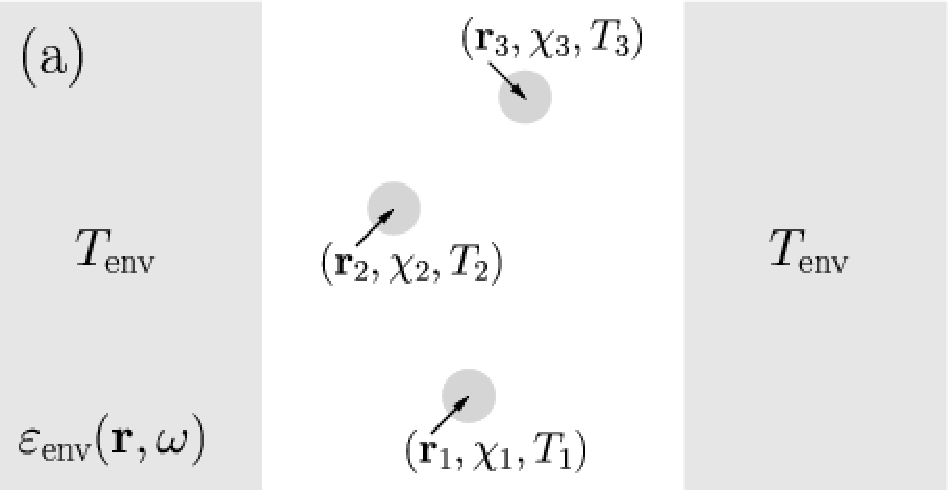
\includegraphics[width=.49\columnwidth]{pics/dipole_pic1a.pdf}
 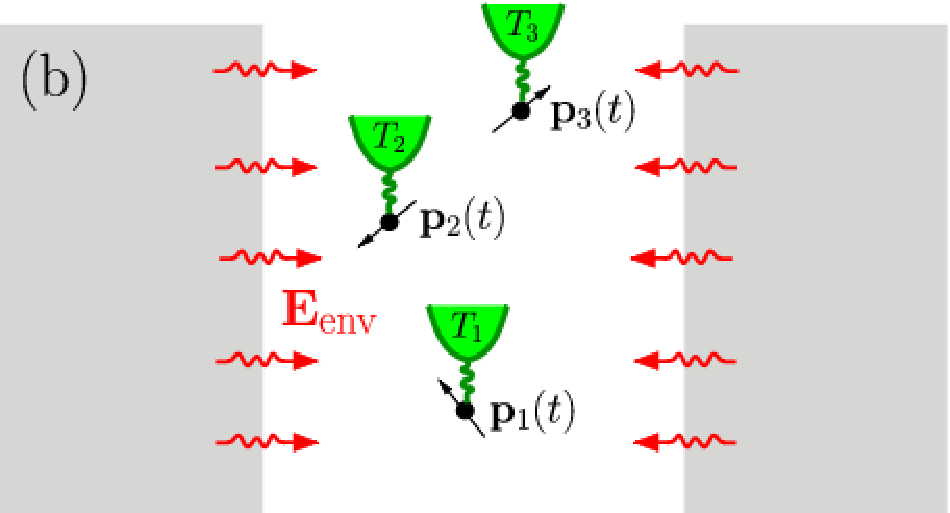
\includegraphics[width=.49\columnwidth]{pics/dipole_pic1b.pdf}
%   \includegraphics[width=.49\columnwidth]{../dipole_resubmission/pic1b}
 \caption{(a) A schematic illustration of the studied system. Small dielectric particles with positions $\mathbf{r}_i$, $i\in\{1,\dots,N\}$, electric susceptibilities $\chi_i(\omega)$ and temperatures $T_i$ are located in an inhomogeneous environment, consisting in the shown case of two dielectric (or metallic) bodies forming a cavity. The overall relative permittivity is $\varepsilon(\br,\omega)=\epsenv(\br,\omega)$ outside the particles and $\varepsilon(\br_i,\omega)=1+\chi_i(\omega)$ at the position of each particle coordinate $\br_i$. The two cavity walls, described by the environment dielectric constans, are assumed to act as a source of thermal radiation at temperature $\Tenv$. The polarization field inside each particle $i$ is modeled as an oscillating point dipole moment $\bb{p}_i$ coupled to a local Langevin heat bath at temperature $T_i$ as depicted in (b). The total local field $\bE(\br_i,t)$ driving each dipole moment $\bb{p}_i$ is the sum of the stochastic background field $\bE_{\textrm{env}}(\br_i,t)$ and the fields $\bE_{ij}(t)$ created by each dipole $j$.}%The local bath temperatures $T_i$ correspond to local lattice temperatures, which could either by given fixed temperatures or could be self-consistently determined by the balance of absorption, emission and the in- and outflow of lattice heat. 
\label{fig:gfm_dipole_system}
\end{figure}

We briefly outline the Langevin equation approach to the electromagnetic energy transfer here (reported in detail in Publication XXX). The studied system is depicted in Fig. \ref{fig:gfm_dipole_system}. Dielectric particles with positions $\mathbf{r}_i$, $i\in\{1,\dots,N\}$ are located in an inhomogeneous environment characterized by the environment's dielectric constant $\epsenv(\br,\omega)$. The overall relative permittivity is then given by $\varepsilon(\br_i,\omega)=1+\chi_i(\omega)$ at the locations of the particles ($\chi_i$ being the electric susceptibility of particle $i$) and $\varepsilon(\br_i,\omega)=\epsenv(\bb{r},\omega)$ elsewhere. For inhomogeneous $\epsenv(\br,\omega)$, the environment acts not only as a source of non-blackbody thermal radiation (at temperature $\Tenv$) but also as a scatterer of the radiation emitted by the particles, thereby modifying the energy transfer rates compared to the free space.

Following the dipole approximation, the internal polarization field of each particle is modeled as a point dipole located at the central coordinate $\br_i$ of the particle $i$ as illustrated in Fig. \ref{fig:sud1}(b). The microscopic dipole moments, which represent the fluctuating electric polarization inside each particle, are then coupled to (1) local heat baths describing thermal fluctuations and dissipation, (2) to the electromagnetic field arising from other dipoles, and (3) to the thermal field originating from the environment.

\subsubsection{Equation of motion and solution}

The local dynamics of each dipole is modeled by the classical oscillator model accompanied by quantum Langevin dynamics. The equation of motion for the local dipole displacement $\bu_i$, related to the dipole moment through $\bp_i=\bu_i/q$ where $q$ is the charge, reads
 \begin{equation}
 m\ddot\bu_i(t) = -m\omega_i^2 \bu_i(t) +\xi_i(t) -m\gamma_i \dot{\bu}_i(t)  + q \bE_i(t). \label{eq:gfm_eom1}
\end{equation}
The oscillator mass $m$, charge $q$, resonance frequency $\omega_i$ and the friction parameter $\gamma_i$ are later absorbed into the definition of the local polarizability. The stochastic force $\xi_i(t)$ is related to the friction term by the standard fluctuation-dissipation relation. The steady state solution to the equation of motion can be again most easily achieved by moving to frequency domain, in which the equations of motion become
\begin{equation}
 -m\omega^2 \hat\bu_i(\omega) = -m\omega_i^2 \hat\bu_i(\omega) +\hat \xi_i(\omega) +im\gamma_i \omega \hat \bu_i(\omega)  + q \hat \bE_i(\omega). \label{eq:gfm_eom2}
\end{equation}

The Fourier transform of the local electric field $\hat \bE_i$ consists of the environment field $\Eenvhat(\br_i,\omega)$ and the fields $\hat \bE_{ij}(\omega)$ generated by each dipole $j$ \cite{novotny}:
\begin{equation}
 \hat{\bE}_i\pom= \Eenvhat(\br_i,\omega) + \sum_{j=1}^N \hat{\bE}_{ij}\pom. \label{eq:gfm_etot}
\end{equation}
The statistical properties of the stochastic environment field are discussed below. The electric field $\bE_{ij}$ due to dipole moment $\hat{\bb{p}}_j$, responsible for the electromagnetic interaction between the dipoles, is given in frequency domain by \cite{novotny}
\begin{equation}
 \hat{\bE}_{ij}(\omega) = \omega^2 \mu_0\gem_{ij}(\omega) \hat{\bp}_j (\omega), \label{eq:gfm_ekl}
\end{equation}
where $\gem_{ij}(\omega)$ is the electromagnetic Green's dyadic found by solving the Helmholtz equation \cite{novotny}
 \begin{equation}
 \nabla \times \nabla \times \gem(\bb{r},\br';\omega) - (\omega^2/c^2) \epsenv(\br,\omega)\gem(\bb{r},\br';\omega)  =  \delta(\bb{r}-\br')\unitdyadic. \label{eq:gemdef}
\end{equation}
in absence of the point dipoles. Here $c$ is the speed of light. The Green's dyadic $\gem$ only accounts for the scattering of the electromagnetic field from the inhomogeneities in the environment. The scattering of the field from the point dipoles is automatically included in the formalism by the coupled dipole equations of motion. The local Green's dyadic $\gem_{ii}(\omega)$, discussed in more detail in Publication XXX, accounts for the Abraham-Lorentz radiation damping, which produces a force term proportional to third time derivative of $\bb{u}$ in the dipole equation of motion \eqref{eq:gfm_eom1}. The fluctuations accompanying the radiation reaction damping are responsible for generating thermal radiation \cite{greffet10}.

The substitution of Eqs. \eqref{eq:gfm_etot} and \eqref{eq:gfm_ekl} to Eq. \eqref{eq:gfm_eom2} gives
\begin{equation}
 -m\omega^2 \hat{\bu}_i \pom =  -m\omega_i^2 \hat \bu_i\pom + \hat{\xi}_i\pom + im\gamma_i \omega \hat{\bu}_i\pom + \Eenvhat(\br_i,\omega) + q^2\omega^2\mu_0 \sum_{j=1}^N \gem_{ij}\pom \hat{\bu}_j\pom. \label{eq:gfm_eom_freq}
\end{equation}
Equation \eqref{eq:gfm_eom_freq} can be rearranged as
\begin{equation}
 - \sum_{j} \bb{A}_{ij} \hat{\bu}_j(\omega) = \hat{\xi}_i(\omega) + q\Eenvhat(\br_i,\omega) \label{eq:gfm_eom_akl}
\end{equation}
by defining an inverse propagator
\begin{equation}
 \bb{A}_{ij} = \left[m(\omega^2-\omega_i^2+i\gamma_i) \right]\delta_{ij}\bb{I}_{3\times 3}+ q^2\omega^2\mu_0 \gem_{ij},
\end{equation}
where $\unitdyadic$ is the $3\times 3$ unit matrix. The solution to Eq. \eqref{eq:gfm_eom_akl} can be written compactly in matrix form as
\begin{equation}
 \hat{\bu}(\omega) = -\bb{G}(\omega) \left[\hat{\xi}(\omega)+q\Eenvhat(\omega) \right], \label{eq:gfm_usol}
\end{equation}
where the dipole displacement Green's function $\bb{G}\pom=\bb{A}\pom^{-1}$ is
\begin{equation}
 \bb{G}(\omega) = \frac{1}{m(\omega^2 \mathbf{I}_{3N\times 3N}-\Omega^2)+q^2\omega^2\mu_0 \textrm{Re}[\gem(\omega)]+i\Gamma^{\textrm{bath}}(\omega)/2+i\Gamma^{\textrm{rad}}(\omega)/2}. \label{eq:gfm_g_expression1}
\end{equation}
Here we adopt a matrix notation where the dipole indices $i\in \{1,\dots,N\}$ and the spatial components $\alpha\in \{1,2,3\}$ are combined into a composite index resulting in matrices and vectors of size $3N\times 3N$ and $3N$, respectively. In the following, we will use an index notation where the subscript $ij$ ($i$) always refers to the $3\times 3$ matrix (3-component vector) corresponding to the notation used before Eq. \eqref{eq:gfm_usol}.

In Eq. \eqref{eq:g_expression1} we have additionally defined the block-diagonal resonance frequency matrix as $\Omega=\textrm{diag}(\omega_1\bb{I}_{3\times 3},\omega_2\bb{I}_{3\times 3},\dots,\omega_N\bb{I}_{3\times 3})$, the block-diagonal bath coupling matrix as $\Gamma^{\textrm{bath}} (\omega) = \textrm{diag}(2m \gamma_1 \omega\bb{I}_{3\times 3},\dots,2m\gamma_N \omega_N \bb{I}_{3\times 3})$,
and the radiation coupling function defined through the imaginary part of the electromagnetic interaction by
\begin{equation}
 \Gamma^{\textrm{rad}}(\omega) = 2 q^2\omega^2\mu_0 \textrm{Im}[\gem(\omega)]. \label{eq:gfm_gammarad_def}
\end{equation}
%In the denominator of Eq. \eqref{eq:g_expression1} and in all matrix-valued expressions appearing below, the scalar terms should be interpreted as being proportional to the unit matrix of size $3N\times3N$.

Equation \eqref{eq:gfm_g_expression1} shows that both the coupling to heat baths and the coupling to the radiation field produce broadening in the Green's function via the coupling functions $\Gamma^{\textrm{bath}}(\omega)$ and $\Gamma^{\textrm{rad}}(\omega)$. This broadening in the Green's function reflects dissipation that, along with the accompanying thermal fluctuations, enables energy transfer between dipoles with different bath temperatures.

\subsubsection{Statistical properties of the background field}

The fluctuation-dissipation theorem for the environment field can be written in the form analogous to Eq. XXX in terms of the radiation coupling function \eqref{eq:gfm_gammarad_def} \cite{novotny}
\begin{alignat}{2}
  q^2 \langle \Eenvhat(\bb{r}_i,\omega) \Eenvhat(\bb{r}_j,\omega')^T \rangle   &=  2\pi \delta(\omega+\omega') \hbar \Gamma^{\textrm{rad}}_{ij}(\omega) \fbbg. \label{eq:gfm_ebgebg1}
\end{alignat}
The simultaneous presence of $\textrm{Im}[\gem_{ij}(\omega)]$ both in Eq. \eqref{eq:gfm_ebgebg1} and as a source of dissipation in the dipole displacement Green's function \eqref{eq:gfm_g_expression1} ensures the onset of thermal equilibrium when the dipole and environment bath temperatures are equal. 

\subsubsection{Heat current}

The heat transfer rates between particles can be inferred from energy conservation arguments. A direct calculation shows that the expectation value of the Poynting vector's flux across a surface $\partial V_i$ enclosing a particle $i$, equal to the power of the emitted radiation field, satisfies 
\begin{equation}
 \left\langle \int_{\partial V_i} \bb{S} \cdot d\bb{S} \right\rangle = - \langle Q_i \rangle,
\end{equation}
where the energy current to the bath is given by the bath force multiplied by the dipole moment ''velocity'': $Q_i = (m\gamma \dot{\bu}_i-\xi_i)\cdot \dot{\bu}_i$. Therefore, $\langle Q_i\rangle$ can be interpreted as the locally absorbed power. Direct calculation carried out in Publication XXX shows that 
\begin{alignat}{2}
 \langle Q_i \rangle &= \int_0^{\infty}\frac{d\omega}{2\pi} \hbar\omega \sum_{j} \ca{T}_{ij}(\omega) \left[f_B(\omega,T_j)-f_B(\omega,T_i ) \right] \notag \\
  & \quad + \int_0^{\infty} \frac{d\omega}{2\pi} \hbar \omega \ca{T}_{i,\textrm{rad}}(\omega)\left[ f_B(\omega,\Tenv)-f_B(\omega,T_i)\right].
\end{alignat}
Here the dipole-dipole transmission function is defined as
\begin{equation}
 \ca{T}_{ij}(\omega) = \textrm{Tr} \left[\Gamma_i(\omega) \bb{G}(\omega) \Gamma_j(\omega) \bb{G}(\omega)^{\dagger} \right]
\end{equation}
and the dipole-environment transmission is 
\begin{equation}
 \ca{T}_{i,\textrm{rad}}(\omega) =  \textrm{Tr} \left\{ \Gamma_i(\omega) \left[ \bb{G}(\omega) \Gamma_{\textrm{rad}}(\omega) \bb{G}(\omega)^{\dagger} \right]_{ii} \right\}.
\end{equation}

\subsubsection{Local polarizabilities}

To calculate the transmission functions, it is useful to express the transmission function in terms of purely optical quantities. This can be achieved by (i) absorbing the microscopic, auxiliary parameters $m$, $q$, $\gamma_i$ to the definitions of the local polarizabilities and (ii) expressing the Green's function in terms of the electromagnetic Green's dyadics. For (i), one must specify the microscopic definition for the polarizability. While there are at least three different definitions available, we use here the Clausius-Mossotti definition 
\begin{equation}
 \langle \hat \bp_i(\omega) \rangle = \varepsilon_0 \alpha_{\textrm{CM}}^i(\omega) \left[\hat \bE_0(\br_i,\omega)+ \left\langle \hat \bE_{\textrm{pol},i} (\omega) \right\rangle \right]
\end{equation}
relating the expectation value of the local dipole moment to the sum of the external field $\bE_0(\br_i,\omega)$ and the polarization field $\bE_{\textrm{pol},i} (\omega)=\hat \bp_i(\omega) /(3\varepsilon_0 \Delta V_i)$ ($\Delta V_i$ is the particle volume). By solving the equation of motion for a single dipole in an external field, one gets 
\begin{equation}
 \alpha_{\textrm{CM}}^i(\omega) = - \frac{q^2}{\varepsilon_0} \frac{1}{m(\omega^2-\omega_i^2+i\gamma_i)-q^2/(3\varepsilon_0\Delta V_i)}\unitdyadic. \label{eq:gfm_alpha_cm_expr}
\end{equation}
One can also start from the microscopic definitions $\varepsilon_i(\omega)=1+\chi_i(\omega)$, $\hat{\bb{P}}(\bb{r}_i,\omega)=\varepsilon_0 \chi_i(\omega) \hat{\bb{E}}(\bb{r}_i,\omega)$ and $\hat{\bb{P}}(\bb{r}_i,\omega)=\hat{\bb{p}}_i(\omega)/\Delta V_i$ to show that
\begin{equation}
 \alpha_{\textrm{CM}}^i(\omega) = 3\Delta V_i \frac{\varepsilon_i(\omega)-1}{\varepsilon_i(\omega)+2} \unitdyadic. \label{eq:alphacm_epsilon}
\end{equation}
Equations \eqref{} and \eqref{} provide the link between the microscopic parameters and the macroscopic dielectric constant $\varepsilon_i(\omega)$ of the particle $i$.

Using Eq. \eqref{eq:} and straightforward albeit tedious algebraic manipulations, one can write the dipole-dipole energy transmission function as
\begin{equation}
   \ca{T}_{ij}(\omega) = 4 \kw^4 \textrm{Tr} \left[ \textrm{Im}[\alpha^i_{\textrm{CM}}(\omega)] \gemfull_{ij}\pom \textrm{Im}[\alpha^j_{\textrm{CM}}(\omega)] \gemfull_{ji}(\omega)^{\dagger}\right]. \label{eq:tij_final}
\end{equation}
Here the electromagnetic Green's dyadic $\gemfull(\omega)$ expressed in terms of the Clausius-Mossotti polarizabilities of the particles has been defined as 
\begin{alignat}{2}
 \gemfull(\omega) &= \frac{1}{\kw^2} \left[\frac{1}{1-\kw^2 \gem(\omega)\alpha_{\textrm{CM}}(\omega)}\right] \alpha_{\textrm{CM}}(\omega)^{-1} \\
  &\equiv \frac{1}{\kw^2} \alpha_{\textrm{CM}}(\omega)^{-1} + \underbrace{ \left[\frac{1}{1-\kw^2 \gem(\omega)\alpha_{\textrm{CM}}(\omega)} \right] \gem(\omega)}_{\tildegemfull}. \label{eq:gfm_gemmb_cm_app}
\end{alignat}
The first term of Eq. \eqref{eq:gfm_gemmb_cm_app} is local and does not contribute to dipole-dipole energy transfer. The second term of Eq. \eqref{eq:gfm_gemmb_cm_app}, denoted by $\tildegemfull$, is non-local and therefore responsible for dipole-dipole energy transfer. By comparing the expression \eqref{} to the one obtained from FED \cite{benabdallah11}, one can show that $\tildegemfull$ is readily interpreted as the electromagnetic Green's dyadic that fully incorporates the scattering caused by the dipoles. %In our manuscript, Eq. \eqref{eq:gfm_gemmb_cm_app} arises as a convenient definition that allows us to express the transmission function \eqref{eq:tij_final} in terms of purely optical quantities.

The radiation transmission function \eqref{eq:tirad} can be similarly written in terms of the polarizabilities and the Clausius-Mossotti Green's dyadic as
\begin{alignat}{2}
 \ca{T}_{i,\textrm{rad}}(\omega) 
 &= 4 \kw^6 \sum_{j,k=1}^N \textrm{Tr}\left\{   \textrm{Im}[\alpha^i_{\textrm{CM}}(\omega)] \gemfull_{ij}(\omega) \alpha_{\textrm{CM}}^j(\omega) \textrm{Im}[\gem_{jk}(\omega)] \alpha^k_{\textrm{CM}}(\omega)^* \gemfull_{ki}(\omega)^{\dagger} \right\}. \label{eq:tirad_final}
\end{alignat}
An equation similar to \eqref{eq:tirad_final} was derived very recently before the publication of Publication XXX by Messina \textit{et al.} \cite{messina13}.

% The thermal background field $\Eenvhat$ has zero average $\langle \Eenvhat \rangle=0$ and its symmetrized autocorrelation function satisfies the fluctuation-dissipation relation 


% \subsection{Introduction to Green's functions}
% 
% \label{sec:gf_linear}
% Green's function method is based on inverting the ''equation of motion operator'', which we will discuss later. For a general non-homogenous equation of the form
% \begin{equation}
%  \mathcal{L} f = g,
% \end{equation}
% where $\mathcal{L}$ is a linear operator and $g$ is the source function, symbolic solution in terms of the Green's function $\mathcal{G}$ is
% \begin{equation}
%  f = \mathcal{G} g.
% \end{equation}
% The Green's function $\mathcal{G}$ is defined as the inverse of $\mathcal{L}$:
% \begin{equation}
%  \mathcal{L} \mathcal{G} = I,
% \end{equation}
% where $I$ is the identity operator. Since $\mathcal{L}$ is linear, solution for 
% \begin{equation}
%  \mathcal{L} f = g_1 + g_2
% \end{equation}
% is the sum of solutions
% \begin{equation}
%  f = \mathcal{G}g_1 + \mathcal{G} g_2.
% \end{equation}
% Calculating $\mathcal{G}$ for a given $\mathcal{L}$ determines, therefore, the solution for any source function $g$. 
% 
% 
% 
% \subsection{Quantum mechanical Green's functions}
% 
% For completeness, we also briefly discuss the Green's functions that appear in the quantum-mechanical many-body problem. These functions are directly defined as statistical averages of different correlation functions and, at first sight, bear no resemblance to the Green's function discussed in Sec. \ref{sec:gf_linear}. The most used two-particle Green's functions are \cite{wang08}
%  \begin{alignat}{2}
%    G^R(t,t') &= -i\theta(t-t') \langle [\bb{u}(t), \bb{u}(t')^T] \rangle \\
%    G^A(t,t') &= i\theta(t'-t) \langle [\bb{u}(t), \bb{u}(t')^T] \rangle\\
%    G^>(t,t') &= -i\langle \bb{u}(t) \bb{u}(t')^T \rangle\\
%    G^<(t,t') &= -i\langle \bb{u}(t') \bb{u}(t)^T \rangle^T	 \\
%    G^t(t,t') &= \theta(t-t') G^>(t,t') + \theta(t'-t) G^<(t,t') \\
%    G^{\bar t}(t,t') &=\theta(t'-t) G^>(t,t') + \theta(t-t') G^<(t,t')  ,
%  \end{alignat}
% which are called the retarded, advanced, greater, lesser, time-ordered and anti-time-ordered Green's functions, respectively. The operators appearing inside the expectation values are written in Heisenberg picture. Out of the six Green's functions, only three are linearly independent and, in steady-state, the number of independent functions is reduced to two. In equilibrium, one of the Green's functions determines the others, and typically $G^R$ is considered. Note that $G^R$ satisfies
% \begin{alignat}{2}
%  \partial_t G^R(t,t')  &= -i \delta(t-t')  \langle [\bb{u}(t), \bb{u}(t')^T] \rangle -i \theta(t-t') \langle [\dot{\bb{u}}(t),\bb{u}(t')^T ] \rangle \\
%   &= -i \theta(t-t') \langle [\bb{p}(t),\bb{u}(t') ]^T \rangle
% \end{alignat}
% and
% \begin{alignat}{2}
%  \partial_t^2 G^R(t,t') &= - i \delta(t-t') \langle [\bb{p}(t),\bb{u}(t') ]^T \rangle - i \theta(t-t') \langle [\dot{\bb{p}}(t),\bb{u}(t')^T] \rangle \\
%   &= - \delta(t-t')\bb{I}  - i \theta(t-t') \langle [\dot{\bb{p}}(t),\bb{u}(t')^T] \rangle .
% \end{alignat}
% For a quadratic Hamiltonian 
% \begin{equation}
%  \mathcal{H} = \frac{\bb{p}^2}{2} + \frac{1}{2} \bb{u}^T \bb{K} \bb{u},
% \end{equation}
% the Heisenberg equation of motion for $\bb{p}(t)$ is 
% \begin{equation}
%  \dot{\bb{p}}(t) = - \bb{K} \bb{u}(t),
%  \label{eq:dotpt}
% \end{equation}
% so 
% \begin{equation}
%  \partial_t^2 G^R_{ij} (t,t') = - \delta(t-t') \delta_{ij} - K_{ik} G^R_{kj}(t,t').
% \end{equation}
% Fourier transformation then gives the familiar Green's function
% \begin{equation}
%  G^R(\omega) = [(\omega+i\eta)^2-\bb{K}]^{-1}
% \end{equation}
% from the last section. This short calculation justifies the name Green's function. Note that for an interacting system, Eq. \eqref{eq:dotpt} would not be valid and the hiearchy of equations of motion would not close.
% 
% The usefulness of Green's functions in the statistical mechanics of quantum-mechanical systems lies in the facts that (1) they can be used to calculate all thermodynamic observables \cite{negele}, and (2) they allow an easy and intuitive perturbative expansion that can be represented as Feynman diagrams \cite{negele,fetter2}. At zero and non-zero temperature, the diagrammatic expansion in terms of the interaction parameter is carried out for the time-ordered Green's function and the Matsubara Green's function, respectively. Methods such as functional renormalization group \cite{metzner12,saaskilahti11} can be applied to sum a subset of diagrams up to an infinite order in a controlled manner.
% 
% In the context of non-equilibrium transport problem, Meir and Wingreen showed that the electronic current through an \textit{interacting} system can be written in terms of $A(\omega)$, the spectral function of the system. Corresponding formula for phonon transport through an anharmonic system was derived by Wang \cite{wang06} and Mingo \cite{mingo06}, and the formula reads for, say, the current flowing to the left lead
% \begin{equation}
%  I = \int \frac{d\omega}{2\pi} \omega \textrm{Tr}\left[G^R(\omega) \Sigma^<(\omega) + G^<(\omega) \Sigma^A(\omega) \right],
% \end{equation}
% where $\Sigma^<$ and $\Sigma^A$ are the lesser and advanced self-energies of the left lead. To calculate the Green's functions and self-energies perturbatively, the perturbation expansion is done for the more general Keldysh Green's function
% \begin{equation}
%  G (\tau,\tau') = -i \langle \mathcal{T}_{\tau} u(\tau) u(\tau') \rangle.
% \end{equation}
% Time variable $\tau$ lies on the Keldysh contour, which runs from $-\infty$ to $\infty$ slightly above the real axis and back to $-\infty$ slightly below the real axis \cite{jauho}.

